\documentclass{beamer}
\usepackage{graphicx}
\usepackage[czech]{babel}
\usepackage[utf8]{inputenc}
\usepackage[T1]{fontenc}
\usepackage{algorithm}
\usepackage{algpseudocode}

\setbeamertemplate{footline}[frame number]

\title{Typografie a~publikování\,--\,5.projekt\\
Binární stromy}
\author{Valentyn Vorobec}
\date{\today}

\begin{document}

\begin{frame}
    \titlepage
\end{frame}

\begin{frame}{Úvod}
    \begin{itemize}
        \item Binární stromy jsou hierarchickou datovou strukturou, která se skládá z uzlů a hran.
        \item Každý uzel má nula až dva potomky: levého a pravého.
        \item Binární stromy se uplatňuje v oblastech informatiky, např. vyhledávání.
    \end{itemize}
\end{frame}

\begin{frame}{Motivace}
    \begin{center}
        \huge Proč se zabývat binárními stromy?
    \end{center}
    \vspace{1em}
    \begin{itemize}
        \item Binární stromy jsou základní datovou strukturou v informatice.
        \item Poskytují efektivní způsob ukládání a organizace dat.
        \item Mají široké uplatnění v algoritmizaci, vyhledávání a řazení.
        \item Porozumění binárním stromům je klíčové pro pochopení pokročilých datových struktur a algoritmů.
    \end{itemize}
\end{frame}

\begin{frame}{Definice}
    \begin{block}{Binární strom}
        Binární strom je buď prázdný, nebo se skládá z kořene a dvou binárních stromů, levý podstrom a pravý podstrom.
    \end{block}
    \begin{figure}
        \centering
        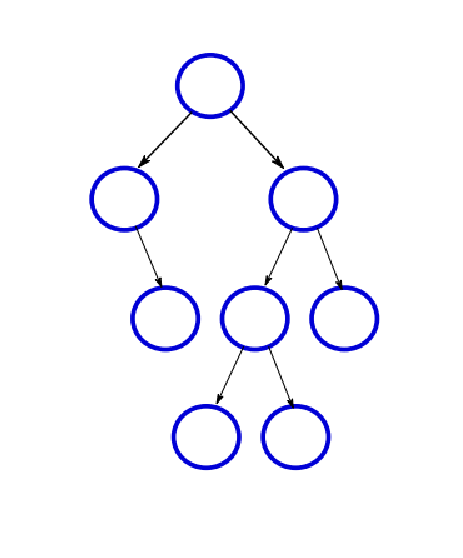
\includegraphics[scale=0.5]{binarni_strom.eps}
        \caption{Příklad binárního stromu.}
    \end{figure}
\end{frame}

\begin{frame}{Výhody a nevýhody}
    \begin{block}{Výhody}
        \begin{itemize}
            \item Efektivní vyhledávaní
            \item Uspořádan průchod
            \item Efektivní využití paměti
            \item Rychlá práce s daty jako vložení a odstranění
            \item Lehká implementace
        \end{itemize}
    \end{block}
    \onslide<2->{
    \begin{block}{Nevýhody}
        \begin{itemize}
            \item Limitovaná struktura
            \item Pomalý výkon v nejhorších scénářích
            \item Prostorová neefektivita
            \item Nevyvážené stromy
            \item Komplexní vyvažovací algoritmy
        \end{itemize}
    \end{block}
    }
\end{frame}

\begin{frame}{Základní operace}
    \begin{enumerate}
        \item \textbf{Vložení (Insertion)}: Vloží nový prvek do stromu.
        \item \textbf{Smazání (Deletion)}: Odebere existující prvek ze stromu.
        \item \textbf{Vyhledávání (Search)}: Najde specifický prvek ve stromu.
        \item \textbf{Průchod (Traversal)}: Projde všechny uzly stromu v určitém pořadí.
    \end{enumerate}
\end{frame}

\begin{frame}{Pseudokód operací}
    \begin{block}{Insertion (Vložení)}
        \begin{itemize}
            \item Pokud je strom prázdný, vytvoříme nový uzel jako kořen.
            \item Jinak porovnáme vkládaný prvek s kořenem a vložíme ho do levého nebo pravého podstromu rekurentně.
        \end{itemize}
        \end{block}

    \begin{block}{Deletion (Smazání)}
        \begin{itemize}
            \item Pokud mazaný uzel nemá žádného potomka, jednoduše ho odstraníme.
            \item Pokud má jeden potomka, nahradíme ho potomkem.
            \item Pokud má oba potomky, nahradíme ho nejbližším pravým potomkem a rekurzivně smažeme ten pravý potomek.
        \end{itemize}
    \end{block}
\end{frame}


\begin{frame}[fragile]{Pseudokód operace - Ukázka}
    \begin{algorithm}[H]
    \caption{Vložení iterativně}\label{alg:bst_insert}
    \tiny
    \begin{algorithmic}[1]
    \Procedure{bst\_insert}{$\text{tree}: \text{ukazatel na ukazatel na uzel}, \text{key}: \text{znak}, \text{value}: \text{celé číslo}$}
        \If{$\text{tree} = \text{NULL}$}
            \State \textbf{return}
        \EndIf
        \State $\text{found} \gets \text{false}$
        \While{$\text{tree} \neq \text{NULL}$ \textbf{and not} $\text{found}$}
            \If{$\text{key} < \text{tree}\rightarrow\text{key}$}
                \State $\text{tree} \gets \text{ukazatel na levý potomek uzlu tree}$
            \ElsIf{$\text{key} > \text{tree}\rightarrow\text{key}$}
                \State $\text{tree} \gets \text{ukazatel na pravý potomek uzlu tree}$
            \Else
                \State $\text{tree}\rightarrow\text{value} \gets \text{value}$
                \State $\text{found} \gets \text{true}$
            \EndIf
        \EndWhile
        \If{$\text{tree} = \text{NULL}$}
            \State Vytvoř nový uzel $\text{new}$
            \If{$\text{new} = \text{NULL}$}
                \State \textbf{return}
            \EndIf
            \State Nastav key uzlu $\text{new}$ na $\text{key}$
            \State Nastav hodnotu uzlu $\text{new}$ na $\text{value}$
            \State Nastav levý potomek uzlu $\text{new}$ na $\text{NULL}$
            \State Nastav pravý potomek uzlu $\text{new}$ na $\text{NULL}$
            \State Nastav $\text{tree}$ na ukazatel na $\text{new}$
        \EndIf
    \EndProcedure
    \end{algorithmic}
    \end{algorithm}
\end{frame}

\begin{frame}{Pseudokód operací (Pokračování)}
    \begin{block}{Search (Vyhledávání)}
        \begin{itemize}
              \item Začneme u kořene.
              \item Porovnáme hledaný prvek s aktuálním uzlem. Pokud jsou stejné, hledání končí.
              \item Pokud je hledaný prvek menší než aktuální uzel, hledáme v levém podstromu; pokud je větší, hledáme v pravém podstromu.
        \end{itemize}
    \end{block}
\end{frame}

\begin{frame}{Složitost operací}
    \begin{itemize}
        \item Vyhledávání, vkládání a mazání v průměru vyžaduje čas \(O(\log n)\), kde \(n\) je počet prvků ve stromě.
        \item Ve špatném případě může dosáhnout časové složitosti \(O(n)\), pokud strom degeneruje do lineární formy.
    \end{itemize}
\end{frame}

\begin{frame}{Zdroje}
    \begin{itemize}
        \item Online materiály:
        \begin{itemize}
            \item \textit{Moodle IAL VUT FIT: Prezentace k přednáškám} [online]. 2022.
        \end{itemize}
        \begin{itemize}
            \item GeeksforGeeks. \textit{Binary Tree Data Structure} [online]. Dostupné z: \\
            \href{https://www.geeksforgeeks.org/binary-tree-data-structure/}{https://www.geeksforgeeks.org/binary-tree-data-structure/}
        \end{itemize}
    \end{itemize}
\end{frame}

\end{document}
